\graphicspath{ {3-SGBD/} }

\chapter{Sistemas Gerenciadores de Banco de Dados}
\label{sgbd}

Antes de se ter um sistema que visava gerenciamento de um banco de dados, era utilizado para persistência de dados o sistema de arquivos. 
Apesar de simples, esta abordagem apresentava alguns problemas por não apresentar suporte à redundância de informações; não garantir integridade de dados; 
falta de segurança; e o acesso e gerenciamento dos dados dependia de programas e aplicativos, fazendo com que seja necessário criar um novo aplicativo, ou adaptá-lo, a 
cada requisição de dados diferente. Outro problema crítico é não se ter informação de relacionamento entre arquivos diferentes.

Como forma de manter o gerenciamento de dados independente de aplicações e programas bem como solucionar os demais falhas do sistema de arquivos 
foram criados os Sistemas Gerenciadores de Bancos de Dados, os SGBD.  De acordo com Elmasri e Navathe \cite{navathe2011banco}, SGBD são uma coleção de programas para 
criação e manutenção de um banco de dados, que facilita a definição, construção, manipulação e compartilhamento de dados entre usuários e aplicações.

Dentre as vantagens que os SGBD trouxeram em detrimento ao sistema de arquivos estão:

\begin{itemize}
    \item{\textbf{Controle de redundância}}, para que não seja permitido duplicação de dados, pois isto causaria desperdício na capacidade de armazenamento.
    \item{\textbf{Restrição de acesso aos usuários}}, pois não será permitida manipulação do banco a todos os usuários, ou funcionários de uma empresa por exemplo.
    \item{\textbf{Execução de consultas eficiente}} através do uso de índices, normalmente implementadas utilizando hash ou árvores, para que o acesso ao disco seja mais rápido.
    \item{\textbf{Restrições de integridade}}, a fim de garantir que (i) dados não sejam inseridos de forma inconsistente de acordo com o tipo de atributo definido; 
    (ii) as relações entre entidades sejam efetuadas e (iii) restrições de chave sejam mantidas.
    \item{\textbf{Persistência de dados}}, para garantir que os dados serão inseridos e de fato armazenados no modelo.
    \item{\textbf{\textit{Backup}}} de dados periodicamente para evitar problemas caso aconteça alguma perda no banco e posterior \textbf{restauração}, para recuperar uma imagem do último backup feito no banco.
\end{itemize}

Existem várias classes de SGBD, conforme sua estruturação e a forma como manipulam os dados, 
entre as mais conhecidas estão o modelo relacional, objeto-relacional, orientado a 
objetos e a abordagem mais recente NoSQL.

\section{SGBD Relacional}

O modelo mais utilizado de SGBD é o relacional, ou SGBDR (SGBD Relacional). Ele foi conceituado por 
Codd \cite{codd1970relational} em 1970 em um artigo no qual são expostas as 
vantagens de um modelo relacional em detrimento a um modelo de redes. 

Um modelo relacional define através de um conjunto de tabelas entidades que representam 
objetos do mundo real, cada qual com seus atributos. Esse conjunto de atributos é 
denominado registro do banco de dados, representando uma tupla, ou linha, na tabela. Assim como no mundo real, 
objetos devem estar também relacionados, e para tal SGBDR utilizam-se de chaves.

Em um SGBDR além de definir relacionamentos, as chaves também garantem integridade entre os dados. 
Existem dois tipos de chaves, uma que garante a unicidade de um atributo, ou seja, assegura que 
não haverão registros repetidos no banco tomando como referência aquele valor de chave, chamada de chave primária (\textit{primary key}, ou PK). A outra chave garante integridade no relacionamento entre duas entidades referenciando uma tabela na outra, que 
é a chave estrangeira (\textit{foreign key}, ou FK).

Tomando como exemplo uma empresa fictícia, são criados dois objetos reais que precisam ser 
representados sob a forma relacional, \textit{funcionário} e \textit{projeto}. Nesta empresa funcionários possuem \textit{nome, 
CPF, sexo, salário,} um \textit{supervisor} e trabalham em um ou mais \textit{projetos}. Esses projetos também possuem atributos: 
\textit{nome, código} e o número do \textit{departamento} no qual foram criados. Apenas com estas informações duas tabelas já são definidas 
no banco, \textit{funcionário} e \textit{projeto}, bem como seus atributos, como ilustra a Figura \ref{fig:func_proj}.

\begin{figure*}[htpb]
	\centering
		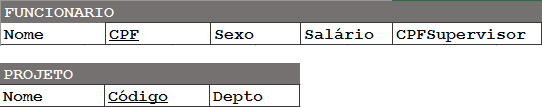
\includegraphics[width=13cm]{funcionario_projeto}
	\caption{Atributos das entidades \textit{funcionário} e \textit{projeto}}
	\label{fig:func_proj}
\end{figure*}

Como descrito, um funcionário trabalha em um ou mais projetos e ele precisa ainda registrar o número 
de horas trabalhadas nestes projetos. Desta forma é preciso de alguma forma relacionar funcionário com os projetos. 
Neste exemplo cabe a criação de uma nova entidade responsável unicamente por relacionar estes dois objetos e ainda 
armazenar o número de horas -- veja que o número de horas não cabe na tabela de funcionários nem na de projetos.

É nesta relação que são explorados os conceitos de chaves em um banco de dados. Para que a entidade que relaciona 
funcionário e projeto tenha informações de que funcionário trabalha em qual projeto é necessário acessar um número, ou código, 
definido para diferenciar todos os funcionários da empresa bem como o código do projeto e relacioná-los. Para o funcionário 
uma PK válida é o número do CPF e para o projeto o próprio atributo código. Essa relação pode ser nomeada unindo 
as entidades que relaciona, nesse caso \textit{funcionário\_projeto}, ou quando faz sentido pode ser nomeada de acordo com a função 
que realiza, neste caso como um funcionário trabalha em um projeto a relação pode ser \textit{trabalha\_em}.

O esquema que representa estas relações é como mostrado na Figura \ref{fig:relacao_func_proj}. Nela podemos ver as chaves primárias, em destaque, nas relações \textit{funcionário} e \textit{projeto}, e seus valores como chave estrangeira na relação \textit{trabalha\_em}. 

\begin{figure*}[htpb]
	\centering
		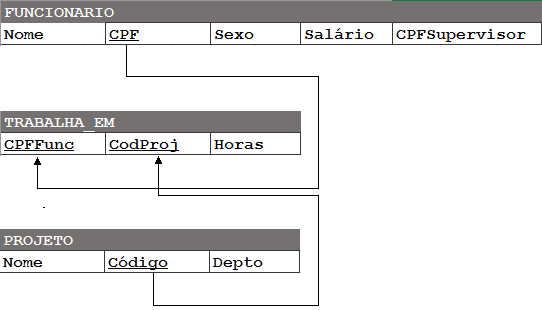
\includegraphics[width=13cm]{relacao_func_proj}
	\caption{Relacionamento entre \textit{funcionário} e \textit{projeto}}
	\label{fig:relacao_func_proj}
\end{figure*}

Modelos de bancos de dados prezam, sempre que possível, pela consistência de dados, principalmente se tomar operações transacionais como transações bancárias, que necessitam de um alto grau de consistência após operações de inserção e atualização, para que não haja perda de valores ou que esses ainda façam sentido no sistema. Por essa razão SGBDR seguem o conceito ACID (Atomicidade, Consistência, Isolamento e Durabilidade). 

Modelos relacionais também seguem um alto grau de normalização nos dados a fim de evitar redundância e confusão entre atributos que podem ser desmembrados em outras entidades. Essa normalização é realizada normalmente até a Terceira Forma Normal (3NF), e o esquema final conterá um número maior de tabelas que o original devido ao desmembramento de atributos. Essa quantidade maior de tabelas acarreta no aumento de junções necessárias para recuperar atributos entre entidades relacionadas, ou seja, no aumento do acesso a entidades e no processamento de tuplas.

Além de diminuir o desempenho na recuperação de dados, um esquema normalizado causa um forte acoplamento entre tabelas, o que tornaria inviável o particionamento dos dados do banco em \textit{n} servidores como forma de escalar estes dados conforme seu volume aumenta (mais detalhes no Capítulo \ref{nosql}), como é o caso de um ambiente analítico. Uma solução trivial para este problema é a denormalização de dados, porém para um SGBDR essa solução pode não ser viável, visto que sua implementação se dá seguindo a modelagem relacional.

Exemplos de SGBDR são PostgreSQL \cite{postgres2018r}, MySQL \cite{mysql2018r}, Microsoft SQL Server \cite{microsoft2018r}, SQLite \cite{lite2018r}, MariaDB \cite{maria2018r} e Oracle \cite{oracle2018r}. 

\section{SGBD NoSQL}

Bancos com o objetivo de suprir problemas apresentados por SGBDR começaram a emergir entre 2004 e 2007 visando alta escalabilidade, recuperação e armazenamento de grandes volumes de dados de forma eficiente, e ao mesmo tempo diminuir custos com hardware \cite{han2011nosql}. Esses bancos levaram o nome de NoSQL, porém isso não significa que não utilizam SQL para manipulação de dados.

Detalhes sobre bancos de dados NoSQL são encontrados no Capítulo \ref{nosql}, no qual também é descrito o modelo colunar, utilizado por satisfazer os requerimentos de um ambiente de DW.